% Figure: Multi-Phase Cache Timeline — Prisoner's Dilemma
% Shows agent cache growth across 5 phases with TTFT annotations

\begin{figure}[t]
\centering
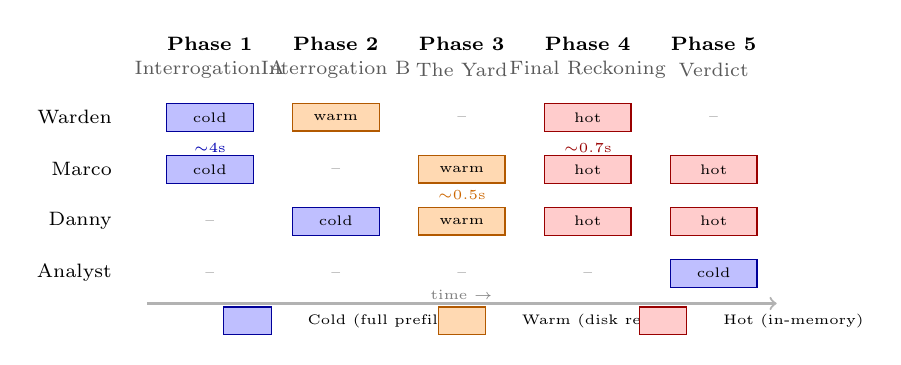
\begin{tikzpicture}[
    x=1.6cm, y=0.55cm,
    phase/.style={rectangle, draw=black, fill=gray!8, minimum height=2.4cm, align=center, font=\scriptsize},
    agent/.style={rectangle, minimum height=0.35cm, font=\tiny, align=center},
    cold/.style={fill=blue!25, draw=blue!60!black},
    warm/.style={fill=orange!30, draw=orange!70!black},
    hot/.style={fill=red!20, draw=red!60!black},
    ttft/.style={font=\tiny, text=black},
    label/.style={font=\scriptsize\bfseries}
]

% Phase labels
\foreach \i/\name/\short in {
    0/{Phase 1}/{\scriptsize Interrogation A},
    1/{Phase 2}/{\scriptsize Interrogation B},
    2/{Phase 3}/{\scriptsize The Yard},
    3/{Phase 4}/{\scriptsize Final Reckoning},
    4/{Phase 5}/{\scriptsize Verdict}} {
    \node[label] at (\i, 5.2) {\name};
    \node[font=\tiny, text=gray!70!black] at (\i, 4.6) {\short};
}

% Agent rows (bottom to top): Warden, Marco, Danny, Analyst
\node[font=\scriptsize, anchor=east] at (-0.7, 3.5) {Warden};
\node[font=\scriptsize, anchor=east] at (-0.7, 2.3) {Marco};
\node[font=\scriptsize, anchor=east] at (-0.7, 1.1) {Danny};
\node[font=\scriptsize, anchor=east] at (-0.7, -0.1) {Analyst};

% Warden: phases 1, 2, 4
\node[agent, cold, minimum width=1.1cm] at (0, 3.5) {cold};
\node[agent, warm, minimum width=1.1cm] at (1, 3.5) {warm};
\node[agent, hot, minimum width=1.1cm] at (3, 3.5) {hot};
% Warden inactive in phase 3, 5
\node[font=\tiny, text=gray] at (2, 3.5) {--};
\node[font=\tiny, text=gray] at (4, 3.5) {--};

% Marco: phases 1, 3, 4, 5
\node[agent, cold, minimum width=1.1cm] at (0, 2.3) {cold};
\node[font=\tiny, text=gray] at (1, 2.3) {--};
\node[agent, warm, minimum width=1.1cm] at (2, 2.3) {warm};
\node[agent, hot, minimum width=1.1cm] at (3, 2.3) {hot};
\node[agent, hot, minimum width=1.1cm] at (4, 2.3) {hot};

% Danny: phases 2, 3, 4, 5
\node[font=\tiny, text=gray] at (0, 1.1) {--};
\node[agent, cold, minimum width=1.1cm] at (1, 1.1) {cold};
\node[agent, warm, minimum width=1.1cm] at (2, 1.1) {warm};
\node[agent, hot, minimum width=1.1cm] at (3, 1.1) {hot};
\node[agent, hot, minimum width=1.1cm] at (4, 1.1) {hot};

% Analyst: phase 5 only
\node[font=\tiny, text=gray] at (0, -0.1) {--};
\node[font=\tiny, text=gray] at (1, -0.1) {--};
\node[font=\tiny, text=gray] at (2, -0.1) {--};
\node[font=\tiny, text=gray] at (3, -0.1) {--};
\node[agent, cold, minimum width=1.1cm] at (4, -0.1) {cold};

% TTFT annotations (below agent boxes)
\node[ttft, text=blue!70!black] at (0, 2.8) {${\sim}4$s};
\node[ttft, text=orange!80!black] at (2, 1.7) {${\sim}0.5$s};
\node[ttft, text=red!60!black] at (3, 2.8) {${\sim}0.7$s};

% Legend
\node[agent, cold, minimum width=0.6cm] at (0.3, -1.2) {};
\node[font=\tiny, anchor=west] at (0.7, -1.2) {Cold (full prefill)};
\node[agent, warm, minimum width=0.6cm] at (2.0, -1.2) {};
\node[font=\tiny, anchor=west] at (2.4, -1.2) {Warm (disk reload)};
\node[agent, hot, minimum width=0.6cm] at (3.6, -1.2) {};
\node[font=\tiny, anchor=west] at (4.0, -1.2) {Hot (in-memory)};

% Time arrow
\draw[->, thick, gray!60] (-0.5, -0.8) -- (4.5, -0.8);
\node[font=\tiny, text=gray] at (2, -0.6) {time $\rightarrow$};

\end{tikzpicture}
\caption{Agent cache state across prisoner's dilemma phases. Permanent agents (Warden, Marco, Danny) start cold and transition to warm/hot as context accumulates via cross-phase injection. Each phase extends the cached prefix rather than re-computing. The Analyst appears only in Phase~5 (cold start). TTFT annotations show projected latency from Table~\ref{tab:ttft} at equivalent context lengths.}
\label{fig:timeline}
\end{figure}
